% Options for packages loaded elsewhere
\PassOptionsToPackage{unicode}{hyperref}
\PassOptionsToPackage{hyphens}{url}
\PassOptionsToPackage{dvipsnames,svgnames,x11names}{xcolor}
%
\documentclass[
  11pt,
  a4paper]{ltjsarticle}
\usepackage{amsmath,amssymb}
\usepackage{iftex}
\ifPDFTeX
  \usepackage[T1]{fontenc}
  \usepackage[utf8]{inputenc}
  \usepackage{textcomp} % provide euro and other symbols
\else % if luatex or xetex
  \usepackage{unicode-math} % this also loads fontspec
  \defaultfontfeatures{Scale=MatchLowercase}
  \defaultfontfeatures[\rmfamily]{Ligatures=TeX,Scale=1}
\fi
\usepackage{lmodern}
\ifPDFTeX\else
  % xetex/luatex font selection
    \setmainfont[]{STIX Two Text}
  \setmathfont[Scale=1.1]{STIX Two Math}
  \ifLuaTeX
    \usepackage[haranoaji,deluxe,no-math]{luatexja-preset}
  \fi
\fi
% Use upquote if available, for straight quotes in verbatim environments
\IfFileExists{upquote.sty}{\usepackage{upquote}}{}
\IfFileExists{microtype.sty}{% use microtype if available
  \usepackage[]{microtype}
  \UseMicrotypeSet[protrusion]{basicmath} % disable protrusion for tt fonts
}{}
\usepackage{xcolor}
\usepackage[includeheadfoot,top=20truemm,bottom=20truemm,right=25truemm,left=25truemm]{geometry}
\usepackage{listings}
\newcommand{\passthrough}[1]{#1}
\lstset{defaultdialect=[5.3]Lua}
\lstset{defaultdialect=[x86masm]Assembler}
\usepackage{longtable,booktabs,array}
\usepackage{calc} % for calculating minipage widths
% Correct order of tables after \paragraph or \subparagraph
\usepackage{etoolbox}
\makeatletter
\patchcmd\longtable{\par}{\if@noskipsec\mbox{}\fi\par}{}{}
\makeatother
% Allow footnotes in longtable head/foot
\IfFileExists{footnotehyper.sty}{\usepackage{footnotehyper}}{\usepackage{footnote}}
\makesavenoteenv{longtable}
\usepackage{graphicx}
\makeatletter
\newsavebox\pandoc@box
\newcommand*\pandocbounded[1]{% scales image to fit in text height/width
  \sbox\pandoc@box{#1}%
  \Gscale@div\@tempa{\textheight}{\dimexpr\ht\pandoc@box+\dp\pandoc@box\relax}%
  \Gscale@div\@tempb{\linewidth}{\wd\pandoc@box}%
  \ifdim\@tempb\p@<\@tempa\p@\let\@tempa\@tempb\fi% select the smaller of both
  \ifdim\@tempa\p@<\p@\scalebox{\@tempa}{\usebox\pandoc@box}%
  \else\usebox{\pandoc@box}%
  \fi%
}
% Set default figure placement to htbp
\def\fps@figure{htbp}
\makeatother
\setlength{\emergencystretch}{3em} % prevent overfull lines
\providecommand{\tightlist}{%
  \setlength{\itemsep}{0pt}\setlength{\parskip}{0pt}}
\setcounter{secnumdepth}{5}
% definitions for citeproc citations
\NewDocumentCommand\citeproctext{}{}
\NewDocumentCommand\citeproc{mm}{%
  \begingroup\def\citeproctext{#2}\cite{#1}\endgroup}
\makeatletter
 % allow citations to break across lines
 \let\@cite@ofmt\@firstofone
 % avoid brackets around text for \cite:
 \def\@biblabel#1{}
 \def\@cite#1#2{{#1\if@tempswa , #2\fi}}
\makeatother
\newlength{\cslhangindent}
\setlength{\cslhangindent}{1.5em}
\newlength{\csllabelwidth}
\setlength{\csllabelwidth}{3em}
\newenvironment{CSLReferences}[2] % #1 hanging-indent, #2 entry-spacing
 {\begin{list}{}{%
  \setlength{\itemindent}{0pt}
  \setlength{\leftmargin}{0pt}
  \setlength{\parsep}{0pt}
  % turn on hanging indent if param 1 is 1
  \ifodd #1
   \setlength{\leftmargin}{\cslhangindent}
   \setlength{\itemindent}{-1\cslhangindent}
  \fi
  % set entry spacing
  \setlength{\itemsep}{#2\baselineskip}}}
 {\end{list}}
\usepackage{calc}
\newcommand{\CSLBlock}[1]{\hfill\break\parbox[t]{\linewidth}{\strut\ignorespaces#1\strut}}
\newcommand{\CSLLeftMargin}[1]{\parbox[t]{\csllabelwidth}{\strut#1\strut}}
\newcommand{\CSLRightInline}[1]{\parbox[t]{\linewidth - \csllabelwidth}{\strut#1\strut}}
\newcommand{\CSLIndent}[1]{\hspace{\cslhangindent}#1}
\ifLuaTeX
\usepackage[bidi=basic]{babel}
\else
\usepackage[bidi=default]{babel}
\fi
\babelprovide[main,import]{japanese}
\ifPDFTeX
\else
\babelfont{rm}[]{STIX Two Text}
\fi
% get rid of language-specific shorthands (see #6817):
\let\LanguageShortHands\languageshorthands
\def\languageshorthands#1{}
\usepackage{luatexja}

\usepackage{tcolorbox}
\usepackage{longtable}
\usepackage{booktabs}
\usepackage{subfig}
\usepackage{ulem}
\usepackage{url}
\usepackage{caption}
\usepackage[backend=biber]{biblatex}
\usepackage{listings}
\usepackage{xcolor}

\lstset{
    basicstyle=\ttfamily,
    keywordstyle=\color[rgb]{0,0,0.6}\bfseries,
    stringstyle=\color[rgb]{0,0.6,0},
    commentstyle=\color[rgb]{0.4,0.4,0.4}\itshape,
    numberstyle=\ttfamily,
    numbers=none,
    stepnumber=1,
    numbersep=15pt,
    numberstyle=\color[rgb]{0.6,0.6,0.6},
    tabsize=4,
    breaklines=true,
    captionpos=t,
    frame=single,
    rulecolor=\color[rgb]{0.8,0.8,0.8}, 
    backgroundcolor=\color[rgb]{0.95,0.95,0.95},
    showspaces=false,
    showtabs=false,
    showstringspaces=false
}

\usepackage{framed}
\usepackage[luatex,unicode]{hyperref}
\hypersetup{
    colorlinks=true,
    linkcolor=black,
    citecolor=black,
    filecolor=black,
    urlcolor=blue
}
\usepackage{pdfpages}
\usepackage{multicol}

\usepackage{siunitx}
\usepackage{fancybox}
\usepackage[version=3]{mhchem}
\AtBeginDocument{\usepackage{physics}}
\usepackage{amsthm}
\usepackage{pgf}
\RequirePackage{luatex85}
\usepackage[all]{xy}
\usepackage{amscd}
\usepackage{tikz-cd}
\usepackage{tikz-feynman}
\usepackage{tikz-feynhand}

\usepackage{mathcommand}
\newmathcommand{\bm}[1]{\symbfit{{#1}}}
\newmathcommand{\slashed}[1]{{\displaystyle{\not}{#1}}}
\renewmathcommand{\d}[1]{\dd{{#1}}}
\renewmathcommand{\~}{\tilde}
\renewmathcommand{\^}{\hat}
\renewmathcommand{\=}{\bar}
\renewmathcommand{\.}{\dot}
\renewmathcommand{\"}{\ddot}

\usepackage{float}
\let\origfigure\figure
\let\endorigfigure\endfigure
\renewenvironment{figure}[1][2] {
    \expandafter\origfigure\expandafter[H]
} {
    \endorigfigure
}

\newenvironment{Shaded}{\begin{shaded}}{\end{shaded}}
\definecolor{shadecolor}{RGB}{200,200,200}
\newenvironment{Highlighting}{}{}

\newcommand{\KeywordTok}[1]{\textcolor[rgb]{0.00,0.44,0.13}{\textbf{{#1}}}}
\newcommand{\DataTypeTok}[1]{\textcolor[rgb]{0.56,0.13,0.00}{{#1}}}
\newcommand{\DecValTok}[1]{\textcolor[rgb]{0.25,0.63,0.44}{{#1}}}
\newcommand{\BaseNTok}[1]{\textcolor[rgb]{0.25,0.63,0.44}{{#1}}}
\newcommand{\FloatTok}[1]{\textcolor[rgb]{0.25,0.63,0.44}{{#1}}}
\newcommand{\CharTok}[1]{\textcolor[rgb]{0.25,0.44,0.63}{{#1}}}
\newcommand{\StringTok}[1]{\textcolor[rgb]{0.25,0.44,0.63}{{#1}}}
\newcommand{\CommentTok}[1]{\textcolor[rgb]{0.38,0.63,0.69}{\textit{{#1}}}}
\newcommand{\OtherTok}[1]{\textcolor[rgb]{0.00,0.44,0.13}{{#1}}}
\newcommand{\AlertTok}[1]{\textcolor[rgb]{1.00,0.00,0.00}{\textbf{{#1}}}}
\newcommand{\FunctionTok}[1]{\textcolor[rgb]{0.02,0.16,0.49}{{#1}}}
\newcommand{\AttributeTok}[1]{\textcolor[rgb]{0.49,0.56,0.16}{#1}}
\newcommand{\RegionMarkerTok}[1]{{#1}}
\newcommand{\ErrorTok}[1]{\textcolor[rgb]{1.00,0.00,0.00}{\textbf{{#1}}}}
\newcommand{\NormalTok}[1]{{#1}}
\newcommand{\VariableTok}[1]{\textcolor[rgb]{0.10,0.09,0.49}{{#1}}}

\setlength{\textwidth}{\fullwidth}
\setlength{\textheight}{40\baselineskip}
\addtolength{\textheight}{\topskip}
\setlength{\voffset}{-0.2in}
\setlength{\topmargin}{0pt}
\setlength{\headheight}{0pt}
\setlength{\headsep}{0pt}
\usepackage{bookmark}
\IfFileExists{xurl.sty}{\usepackage{xurl}}{} % add URL line breaks if available
\urlstyle{same}
\hypersetup{
  pdftitle={イントロダクション},
  pdfauthor={GPT-4o},
  pdflang={ja},
  colorlinks=true,
  linkcolor={blue},
  filecolor={Maroon},
  citecolor={Blue},
  urlcolor={Blue},
  pdfcreator={LaTeX via pandoc}}

\title{イントロダクション}
\author{GPT-4o}
\date{\today}

\begin{document}
\maketitle

このドキュメントは、Pandocを使用してMarkdownからPDFに変換する際のスタイルを確認するための物理学に関連したサンプルです。ChatGPTに吐かせたサンプルですので、内容の正確さに関しては一切保証しません。

\section{外部ファイルの挿入}\label{ux5916ux90e8ux30d5ux30a1ux30a4ux30ebux306eux633fux5165}

外部ファイルを挿入する例を示します。

\section{力学の基本}\label{ux529bux5b66ux306eux57faux672c}

力学は物理学の基礎であり、物体の運動と力の関係を研究する分野です。この章では、ニュートンの運動の法則について学びます。

\subsection{ニュートンの第一法則}\label{ux30cbux30e5ux30fcux30c8ux30f3ux306eux7b2cux4e00ux6cd5ux5247}

ニュートンの第一法則は、「慣性の法則」とも呼ばれ、次のように述べられます。

\begin{tcolorbox}

\textbf{ニュートンの第一法則}:\\
「外力が作用しない限り、静止している物体は静止し続け、運動している物体はその運動を続ける」

\end{tcolorbox}

この法則は、物体が外力を受けない限り、その運動状態を維持しようとする性質(慣性)を表しています。

\subsection{ニュートンの第二法則}\label{ux30cbux30e5ux30fcux30c8ux30f3ux306eux7b2cux4e8cux6cd5ux5247}

ニュートンの第二法則は、「運動の法則」とも呼ばれ、力と運動の関係を次のように示します。

\[
\vec{F} = m\vec{a}
\]

ここで、\(\vec{F}\)は力、\(m\)は質量、\(\vec{a}\)は加速度です。この式は、力が物体に与える影響を定量的に表現しています。

\subsection{ニュートンの第三法則}\label{ux30cbux30e5ux30fcux30c8ux30f3ux306eux7b2cux4e09ux6cd5ux5247}

ニュートンの第三法則は、「作用反作用の法則」として知られ、次のように述べられます。

\begin{proof}[\textbf{証明}]

\textbf{ニュートンの第三法則}:\\
「すべての作用にはそれに等しい反作用がある」

\end{proof}

この法則は、物体が他の物体に力を加えると、その物体も同じ大きさで反対方向の力を返すことを意味します。

\section{エネルギー保存の法則}\label{ux30a8ux30cdux30ebux30aeux30fcux4fddux5b58ux306eux6cd5ux5247}

エネルギー保存の法則は、物理学において非常に重要な原理であり、エネルギーは形を変えても常に保存されることを示します。

\subsection{運動エネルギーと位置エネルギー}\label{ux904bux52d5ux30a8ux30cdux30ebux30aeux30fcux3068ux4f4dux7f6eux30a8ux30cdux30ebux30aeux30fc}

物体の運動エネルギーと位置エネルギーについて学びます。

\subsubsection{運動エネルギー}\label{ux904bux52d5ux30a8ux30cdux30ebux30aeux30fc}

運動エネルギーは、運動する物体が持つエネルギーであり、次の式で表されます。

\[
K = \frac{1}{2}mv^2
\]

ここで、\(K\)は運動エネルギー、\(m\)は質量、\(v\)は速度です。

\subsubsection{位置エネルギー}\label{ux4f4dux7f6eux30a8ux30cdux30ebux30aeux30fc}

位置エネルギーは、物体がある位置にあることによって持つエネルギーであり、次の式で表されます。

\[
U = mgh
\]

ここで、\(U\)は位置エネルギー、\(m\)は質量、\(g\)は重力加速度、\(h\)は高さです。

\subsection{エネルギー保存の法則}\label{ux30a8ux30cdux30ebux30aeux30fcux4fddux5b58ux306eux6cd5ux5247-1}

エネルギー保存の法則は、エネルギーの総量が時間の経過に関係なく一定であることを示します。この法則は次のように表現されます。

\begin{tcolorbox}

\textbf{エネルギー保存の法則}:\\
「孤立系におけるエネルギーの総量は常に一定である」

\end{tcolorbox}

これにより、エネルギーが形を変えても、その総量は変わらないことが確認できます。

\subsection{機械的エネルギーの保存}\label{ux6a5fux68b0ux7684ux30a8ux30cdux30ebux30aeux30fcux306eux4fddux5b58}

運動エネルギーと位置エネルギーを合わせた機械的エネルギーは、摩擦などの外力がない限り、常に一定であることが知られています。これを「機械的エネルギー保存の法則」と呼びます。

\section{Pythonを使った数値解析の例}\label{pythonux3092ux4f7fux3063ux305fux6570ux5024ux89e3ux6790ux306eux4f8b}

ニュートン法を用いて関数の根を求めるPythonコードの例を示します。

\begin{lstlisting}[language=Python]
import numpy as np

def f(x):
    return x**2 - 2

def df(x):
    return 2*x

def newton_method(x0, tol=1e-10, max_iter=100):
    x = x0
    for i in range(max_iter):
        x_new = x - f(x)/df(x)
        if abs(x_new - x) < tol:
            break
        x = x_new
    return x

root = newton_method(1.0)
print(f"squred 2: {root}")
\end{lstlisting}

\section{力学におけるベクトル場の描画}\label{ux529bux5b66ux306bux304aux3051ux308bux30d9ux30afux30c8ux30ebux5834ux306eux63cfux753b}

TikZを使用して二次元のベクトル場を描画する例を示します。

\begin{figure}
\centering
\begin{tikzpicture}
\draw[->] (-2,0) -- (2,0) node[below right] {$x$};
\draw[->] (0,-2) -- (0,2) node[above left] {$y$};
\foreach \x in {-1.5,-1,...,1.5}
    \foreach \y in {-1.5,-1,...,1.5}
        \draw[->, blue] (\x,\y) -- (\x+0.5*\x,\y+0.5*\y);
\end{tikzpicture}
\end{figure}

\section{量子力学におけるシュレディンガー方程式}\label{ux91cfux5b50ux529bux5b66ux306bux304aux3051ux308bux30b7ux30e5ux30ecux30c7ux30a3ux30f3ux30acux30fcux65b9ux7a0bux5f0f}

量子力学の基本方程式であるシュレディンガー方程式を数式として表示します。

\begin{tcolorbox}

時間依存シュレディンガー方程式は次のように表されます。

\[
i\hbar \frac{\partial \psi(x,t)}{\partial t} = \left( -\frac{\hbar^2}{2m} \nabla^2 + V(x) \right) \psi(x,t)
\]

ここで、\(i\)は虚数単位、\(\hbar\)はディラック定数、\(\psi(x,t)\)は波動関数、\(V(x)\)はポテンシャルエネルギーです。

\end{tcolorbox}

\section{証明の例}\label{ux8a3cux660eux306eux4f8b}

数学的な証明を示します。

\begin{proof}[\textbf{証明}]

ベクトルの内積は次のように定義されます。

\[
\vec{a} \cdot \vec{b} = |\vec{a}| |\vec{b}| \cos\theta
\]

ここで、\(\theta\)はベクトル\(\vec{a}\)と\(\vec{b}\)の間の角度です。この定義から、内積が0になる条件は\(\theta = \frac{\pi}{2}\)すなわち、ベクトル\(\vec{a}\)と\(\vec{b}\)が直交する場合です。

\end{proof}

\section{実験データの可視化}\label{ux5b9fux9a13ux30c7ux30fcux30bfux306eux53efux8996ux5316}

以下に、実験データを表形式で示します。これは、ある物理実験で得られたデータです。

\begin{longtable}[]{@{}ll@{}}
\toprule\noalign{}
時間 (s) & 距離 (m) \\
\midrule\noalign{}
\endhead
\bottomrule\noalign{}
\endlastfoot
0.0 & 0.0 \\
1.0 & 9.8 \\
2.0 & 19.6 \\
3.0 & 29.4 \\
4.0 & 39.2 \\
\end{longtable}

\section{実験装置の構造図}\label{ux5b9fux9a13ux88c5ux7f6eux306eux69cbux9020ux56f3}

以下に、実験装置の構造を図として示します。

\begin{figure}
\centering
\pandocbounded{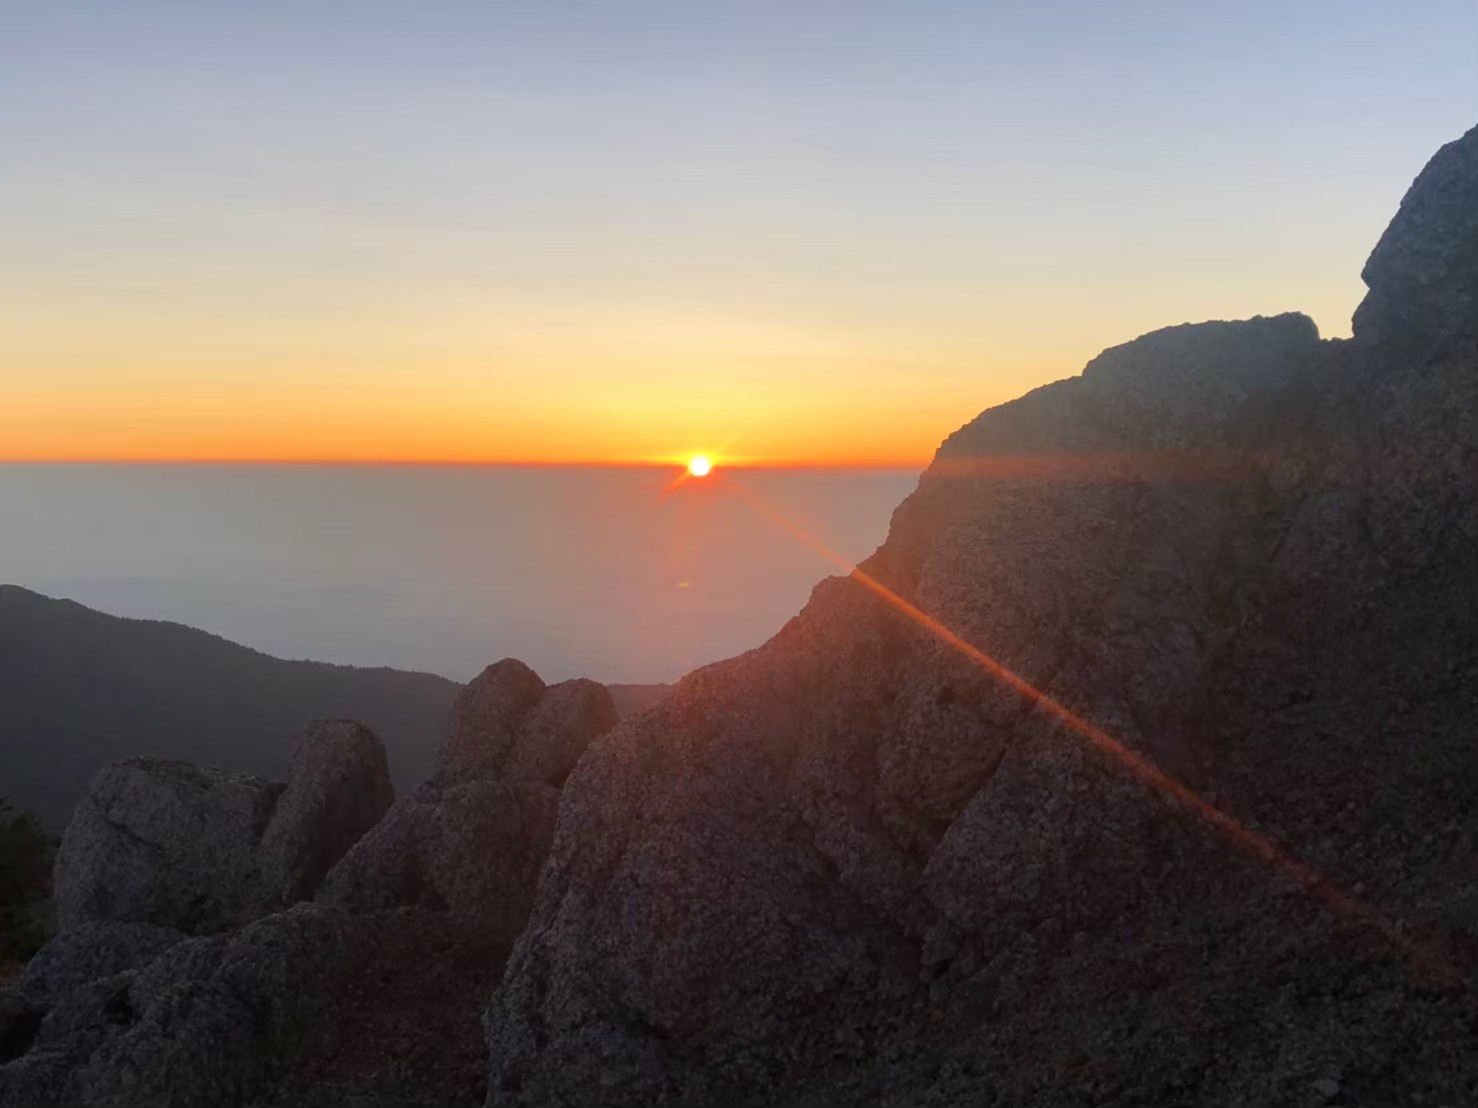
\includegraphics[keepaspectratio]{./test.jpg}}
\caption{実験装置の構造図}
\end{figure}

\section{文献引用の例}\label{ux6587ux732eux5f15ux7528ux306eux4f8b}

物理学の理論は多くの文献に基づいています。たとえば、次のように文献を引用できます
{[}1{]}.

複数個の文献を引用することも可能です{[}2{]} {[}3{]}.

\section{関連リンク}\label{ux95a2ux9023ux30eaux30f3ux30af}

さらに詳しい情報が必要な場合は、\href{https://en.wikipedia.org/wiki/Quantum_mechanics}{量子力学のWikipediaページ}をご覧ください。

\section*{参考文献}\label{ux53c2ux8003ux6587ux732e}
\addcontentsline{toc}{section}{参考文献}

\phantomsection\label{refs}
\begin{CSLReferences}{0}{0}
\bibitem[\citeproctext]{ref-sample1}
\CSLLeftMargin{{[}1{]} }%
\CSLRightInline{ore. Title of the Paper. Journal Name. 2024, vol. 12,
no. 3, p. 123--130.}

\bibitem[\citeproctext]{ref-sample2}
\CSLLeftMargin{{[}2{]} }%
\CSLRightInline{watashi. Title of the Paper. Journal Name. 2024, vol.
12, no. 3, p. 123--130.}

\bibitem[\citeproctext]{ref-sample3}
\CSLLeftMargin{{[}3{]} }%
\CSLRightInline{僕. Title of the Paper. Journal Name. 2024, vol. 12, no.
3, p. 123--130.}

\end{CSLReferences}

\end{document}
